\chapter{Same-Sign W-boson Scattering Analysis}
\label{ssWW_analysis}
\section{Overview of Background Contributions}
Despite being distinctive, the experimental signature of same-sign W-boson scattering: $\ell^{\pm}\ell^{\pm} + jj + E_{T}^{miss}$, can still be faked by other Standard Model processes. These Standard Model background processes can be considered as falling into one two categories:
\begin{enumerate}
\item background processes where one or both leptons originate from jets or photons,
\item and all other background contributions, which can be sub-categorised as:
	\begin{enumerate}
	\item background processes that really do produce two same-sign leptons,
	\item and background processes that produce opposite-sign leptons where one of the leptons' charge is misidentified during reconstruction.
	\end{enumerate}
\end{enumerate}
Background contributions are also classified into prompt and non-prompt backgrounds. Leptons coming from a W-boson are said to be prompt (making up the prompt background), while those coming from the decay of a hadron or a $\uptau$-lepton are said to be non-prompt (making up the non-prompt background).

Expanding upon the above classifications, same-sign W-boson scattering backgrounds can be specifically associated with three sources:
\begin{itemize}
\item Backgrounds resulting from jet-faked leptons are examples of category 1. These are processes in which one or two jets are misreconstructed as leptons or give rise to non-prompt leptons. Lepton quality and isolation requirements, as well as the $b$-jet veto and $E_{T}^{miss}$ requirements are used to suppress such processes, including: $W$ + $jets$, $t\bar{t}$, single top, or QCD multijet processes. Additionally, $W\gamma$ + $jets$ processes where the photon is misreconstructed as an electron, are also an example from category 1. Lepton quality, isolation requirements, and a veto on any events with a third lepton are used for suppression.
\item Processes where three or four leptons are produced, but only two leptons are reconstructed, are examples of sub-category 2.a. This can happen in the case of $WZ$ + $jets$ where the lepton from the W decay and the same-sign lepton from the Z decay pass all selection requirements while the remaining lepton is not reconstructed.
\item Background contributions resulting from charge misidentification (mis-ID) are examples of sub-category 2.b. These are opposite-sign processes where the sign of one lepton is misreconstructed. This can happen due to bremsstrahlung, where an lepton radiates a high energy photon which then pair produces with one of the resulting leptons reconstructed. The power radiated is proportional to $m^{-4}$ for when acceleration is perpendicular to the direction of motion, and $m^{-6}$ for when acceleration is parrallel to the direction of motion \cite{brem}; where $m$ is the particle's mass. In reality, any accelerating particle will have components of its acceleration both perpendicular and parrallel to its motion. However, even for motion that is purely perpendicular to the acceleration, as is the case in circular motion, heavier particles will radiate less than lighter particles (since the power radiated is still proportional to $m^{-4}$). Due to this mass dependence, electrons tend to radiate more energy than the heavier muons. The charge misidentification rate is hence higher for electrons than muons. Processes that contribute to the charge misidentification background include: $t\bar{t}$ \footnote{$t\bar{t}$ processes contribute to both of our two main categories. Semi-leptonic $t\bar{t}$ decays contribute to the non-prompt background (part of category 1), while in other cases, where the top quarks decay fully leptonically, they contribute to they contribute to the prompt background (part of the second category 2.). The two prompt leptons produced in the fully leptonic decay will be opposite-sign rather than same-sign, so this background comes from charge misidentification.}, $W^{\pm}W^{\pm}$ + $jets$, and $Z/\gamma^{*}$ + $jets$ $\longrightarrow \ell^{\pm}\ell^{\pm}$ + $jets$. A veto on events in which a $b$-jet is tagged ($b$-jet veto) is used to help suppress contributions from $t\bar{t}$, while a Z-mass veto is used to suppress $Z/\gamma^{*} \longrightarrow e^{+}e^{-}$, in the $ee$ channel.
\end{itemize}
\section{Object Selection}
\label{object_selection}
Physics objects in the analysis of same-sign W-boson scattering events are required to pass selection requirements in order to help suppress backgrounds coming from other Standard Model processes. This section describes the criteria for objects relevant to same-sign W-boson scattering analysis, i.e. electrons, muons, jets, and overlap removal.
\subsection{Triggers}
The high-level trigger is configured to trigger on electrons that have $p_{T} \geq 24$ GeV and pass the medium electron quality requirements, or alternatively, $p_{T} > 120$ GeV and pass the loose muon quality requirements. Muons trigger on $p_{T} > 50$ GeV, or on $p_{T} > 20$ GeV provided the muon also passes a loose isolation requirement (see \cite{trigger} for details).
\subsection{Muons}
Kinematic cuts are employed in order to reduce the contribution of muons from pile-up collisions and the multijet background. A given muon candidate is required to have an associated track in the inner detector that originates from the primary vertex. In practice this is done by requiring that the muon's flight path intersects the beam axis (z-axis) within 0.5 mm of the primary vertex and that the $d_{0}$ significance is less than 3. Furthermore, the muon is required to have a $p_{T} > 25$ GeV, and fall within a geometrical acceptance of $| \eta | < 2.5$. The $ | \eta | $ requirement corresponds to the total coverage of the precision-tracking (pixel and SCT) detectors. A muon candidate must also pass the default identification requirement, which only allows stand-alone or combined tracks (see section \ref{muon_reco}). These requirements are summarised in table \ref{tight_muon}.

\begin{table}[h]
	\centering{
	\begin{tabular}{c}
	Muon Selection \\ \hline \hline
	Identification: stand-alone or combined tracks \\ \hline
	Isolation: \textit{Gradient} \\ \hline
	Kinematic Acceptance: $p_{T} > 27$ GeV \\ \hline
	Geometrical Acceptance: $| \eta | < 2.5$ \\ \hline
	Longitudinal Impact parameter requirement: $| z_{0} \times \sin \theta | < 0.5$ mm \\
	Transverse Impact parameter requirement: $\frac{d_{0}}{\sigma_{d_{0}}} < 3$ \\ \hline \hline
	\end{tabular}}
	\caption{Signal muon definition}
	\label{tight_muon}
\end{table}

In the implementation of the third lepton veto (see section \ref{event_selection}), a looser selection criteria is applied to candidate veto muons; see table \ref{loose_muon}.

\begin{table}[h]
	\centering{
	\begin{tabular}{c}
	Muon Selection \\ \hline \hline
	Identification: stand-alone or combined tracks \\ \hline
	Isolation: \textit{LooseGradient} \\ \hline
	Kinematic Acceptance: $p_{T} > 10$ GeV \\ \hline
	Geometrical Acceptance: $| \eta | < 2.5$ \\ \hline
	Longitudinal Impact parameter requirement: $| z_{0} \times \sin \theta | < 0.5$ mm \\
	Transverse Impact parameter requirement: $\frac{d_{0}}{\sigma_{d_{0}}} < 3$ \\ \hline \hline
	\end{tabular}}
	\caption{Veto muon definition}
	\label{loose_muon}
\end{table}

\subsection{Electrons}
Electrons are reconstructed using energy deposits in the calorimeter together with the associated matched tracks in the inner-detector. Candidates are required to pass the tight cut definition selection criteria, described in section \ref{electron_reco}, and encompasses cuts based on shower shape, track quality, detection of transition radiation, and track-to-calorimeter-cluster matching (see tight cuts selection in section \ref{electron_reco}). Additional requirements include $p_{T} > 27$ GeV, and a geometrical acceptance of $| \eta | < 1.37$. Note that the $ | \eta | $ requirement restricts electron reconstruction to the barrel region of the electromagnetic calorimeter. These requirements are summarised in table \ref{tight_electron}.

\begin{table}[h]
	\centering{
	\begin{tabular}{c}
	Electron Selection \\ \hline \hline
	Identification: tight cut selection \\ \hline
	Isolation: \textit{Gradient} \\ \hline
	Kinematic Acceptance: $p_{T} > 27$ GeV \\ \hline
	Geometrical Acceptance: $| \eta | < 1.37$ \\ \hline
	Longitudinal Impact parameter requirement: $| z_{0} \times \sin \theta | < 0.5$ mm \\
	Transverse Impact parameter requirement: $\frac{d_{0}}{\sigma_{d_{0}}} < 5$ \\ \hline \hline
	\end{tabular}}
	\caption{Signal electron definition}
	\label{tight_electron}
\end{table}

\begin{table}[h]
	\centering{
	\begin{tabular}{c}
	Electron Selection \\ \hline \hline
	Identification: medium cut selection\\ \hline
	Isolation: \textit{LooseGradient} \\ \hline
	Kinematic Acceptance: $E_{T} > 10$ GeV \\ \hline
	Geometrical Acceptance: $| \eta | < 2.47$, outside crack region $1.37 \geq | \eta | \geq 1.52$ \\ \hline
	Longitudinal Impact parameter requirement: $| z_{0} \times \sin \theta | < 0.5$ mm \\
	Transverse Impact parameter requirement: $\frac{d_{0}}{\sigma_{d_{0}}} < 5$ \\ \hline \hline
	\end{tabular}}
	\caption{Veto electron definition}
	\label{loose_electron}
\end{table}

Like muons, candidate veto electrons (for the third lepton veto) are subjected to a looser a set of requirements. They are only require to pass the medium selection cuts, given in section \ref{electron_reco}. See table \ref{loose_electron} for summary.
\subsection{Jets}
Jets are reconstructed using the \emph{anti-$k_{t}$} algorithm from topological calorimeter clusters. The jets are then calibrated from the electromagnetic energy scale to the hadronic energy scale using a correction factor \cite{JetCorrection}, dependent on $E_{T}$ and $\eta$, from Monte Carlo simulations. A same-sign W-boson scattering event results in two forward jets. Therefore event candidates must have at least two jets with $p_{T} > 30$ GeV and $| \eta | < 4.5$. The two jets with the highest $p_{T}$ are designated the tagging jets.
\subsection{Overlap Removal}
It is possible for a single physics object to be reconstructed multiple tines and, conversely, for two distinct objects may be sufficiently spatially overlap that they are misreconstructed as a single object. The overlap removal procedure is intended to reduce such instances. The overlap procedure used in this analysis is that followed by the Analysis Harmonisation Group \cite{OLR}, and examines and removes objects in a pre-defined order, described as follows:
\begin{enumerate}
\item electron/jet: If the calorimeter cluster associated with an electron, overlaps with that of a jet within $\Delta R =0.3$, both objects are removed.
\item electron/muon: A muon may be misreconstructed as an electron if it's associated track in the I.D. is matched to an electromagnetic cluster resulting from bremsstrahlung. Hence, if a reconstructed electron lies within $ \Delta R =0.1$ of a reconstructed muon, the electron is removed.
\item As previously mentioned, muons coming from the decay of a hadron are part of the non-prompt background. Hence, any muon found to be within $\Delta R =0.3$ of a jet results in the whole event being vetoed.
\end{enumerate}
\section{Event Selection}
\label{event_selection}
In addition to applying a selection criteria to same-sign W-boson scattering candidate objects in order to reduce backgrounds from other Standard Model processes, additional requirements are imposed on candidate events in order to further suppress undesirable background contributions. To this end a series of cuts are applied to candidate events:
\begin{enumerate}
\item any event in which the primary vertex has less than three associated tracks is vetoed,
\item exactly two leptons with $m_{\ell \ell '} > 20$ GeV,
\item any events with additional leptons are excluded (third lepton veto),
\item $q_{\ell _{1}} \times q_{\ell _{2}} > 0$ (same-sign),
\item $|m_{ee} - m_{Z}| > 15$ GeV ($ee$ channel only),
\item $E_{T}^{miss} \geq 10$ GeV,
\item a minimum of two jets with $p_{T} > 30$ GeV and $|\eta | < 4.5$,
\item $b$-jet veto using the ATLAS Run 2 multivariate b-tagger with the $70\%$ working point,
\item $m_{jj} \geq 500$ GeV,
\item $| \Delta y_{jj} | > 2.3$.
\end{enumerate}

Cut 1 involves cleaning cuts applied to events that pass the \textsc{HLT}, including: vetoing incomplete events, requiring at least one vertex with at least three associated tracks with $p_{T} > 0.5$ GeV, cleaning of jets\footnote{Jet cleaning is the process of applying some selection criteria to remove jets that may be fake (sources of fake jets include LHC beam conditions, known hardware malfunctions, and coming from cosmic ray showers), or are likely to be mismeasured \cite{jet_cleaning}.}, and \textsc{GRL} (Good Runs List\footnote{A luminousity block is a time period of approximately two minutes associated with data taking. The Good Runs List is used to select only ``good'' luminousity blocks. ``Bad'' luminousity blocks are those that do not contain viable data for a variety of regions, e.g. sub-detectors were switched off, the LHC beam was not stable, or the magnets were off or ramping.}) selection.

Cuts 2 to 4 correspond to selecting events with exactly two same-sign leptons. The invariant mass requirement is used to reduce the uncertainty in modelling low mass Drell-Yan\footnote{A Drell-Yan process is a process in which a quark and an antiquark (from distinct hadrons) annihilate, creating a virtual $\gamma/Z$ which then decays to a pair of opposite-sign leptons.} processes.

Cut 5 is a Z-mass veto cut intended to reduce the Drell-Yan background $Z \longrightarrow ee$, where one of the lepton's charges is misreconstructed.

The pair of escaping neutrinos carry away some transverse energy. Hence cut 6 cuts out events that lack sufficient $E_{T}^{miss}$ to be from a same-sign W-boson scattering event.

Cut 8, a $b$-jet veto, is used to reduce background contributions coming from top processes.

The last two cuts deal with the forward tagging jets. They are required to have an invariant mass of at least 500 GeV (cut 9), and be separated in rapidity by at least 2.4 (cut 10 ).
\section{Fake Lepton Background}
\label{intro_to_flb}
Non-prompt leptons, which result from the decay of a hadron together with jets misreconstructed as leptons, are referred to as jet-faked leptons. Processes where a prompt lepton is reconstructed along with a jet-faked lepton contribute to background in events selected for measurement of same-sign W-boson scattering. This background is subsequently referred to as the jet-faked lepton background or simply \emph{fake lepton background}. Dominant contributions to the fake lepton background come from $W$ + $jets$, $t\bar{t} \longrightarrow WbWb \longrightarrow \ell \nu bb qq$, and single top processes. In each case a W-boson decays leptonically with the second lepton being jet-faked. The degree to which leptons are isolated (see section \ref{isolation_section}) can be used to reduce the fake lepton background.

Some common processes which contribute to the \emph{fake lepton background} involve the decay of a top quark to a bottom quark by emission of a $W^{+}$, e.g. a semi-leptonic $t\bar{t}$ process (see figure \ref{semi-leptonic_ttbar}). Top-quarks overwhelmingly decay to bottom-quarks through emission of a W-boson \cite{PDG}. Thus implementing a veto on any event that is found to contain a b-jet can help suppress the fake lepton background.

\begin{figure}
\centering{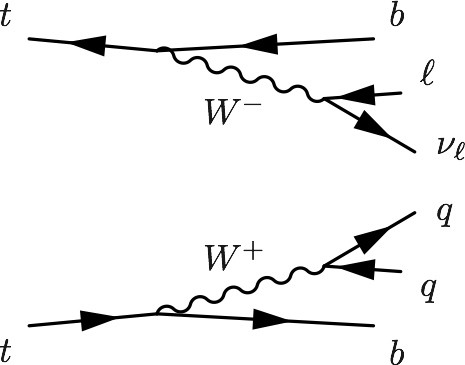
\includegraphics[scale=0.5]{images/semi-leptonic_ttbar.png}}
\caption{Feynman diagram for a semi-leptonic $t\bar{t}$ decay. In same-sign W-boson scattering such processes can contribute to the fake lepton background if one of the resulting jet is misreconstructed as a lepton of the same-sign as the other reconstructed lepton.}
\label{semi-leptonic_ttbar}
\end{figure}